\documentclass[12pt]{article} 
\usepackage{graphics}
\usepackage{setspace}
\usepackage{cite}

% the following is to get inch margins on a letter-size paper
\setlength{\topmargin}{0pt}
\setlength{\headheight}{0in}
\setlength{\headsep}{0in}
\setlength{\textheight}{9.0in}
\setlength{\footskip}{0.5in}
\setlength{\oddsidemargin}{0pt}
\setlength{\evensidemargin}{0pt}
\setlength{\textwidth}{6.5in}

\doublespacing
\begin{document}
\title{A Java Wrapper For Embarrassingly Parallel Problems}
\author{Jacob Schwartz}
\maketitle

\begin{abstract}
An embarrassingly parallel problem, also called pleasingly parallel, is one that 
can be easily broken up into identical components that do not need to interact 
to find the solution. Several problems in the biological sciences are 
embarrassingly parallel but they are difficult to rewrite to use multithreading, 
because they are either poorly written or too complex. We have written a 
framework, implemented in Java, that will execute the serial program in several 
threads. These threads working together help cut down the total runtime of the
program exponentially. The next step is to separate the framework into a 
front-end that will run locally and a back-end which receives blocks of work and 
does the computations. This back-end should run in the cloud, on a machine that 
is dedicated to running embarrassingly parallel tasks only.
\end{abstract}

\section{Introduction}

A computation graph consists of nodes that represent the functions or processes. 
The edges of the graph show data being passed from one process to another. If 
the graph is disconnected, none of the processes need to communicate to complete
the computations. Such a computation is called "embarrassingly parallel." In a 
practical situation, there will be some inter-node communication to set up the 
problem, and then again to accumulate the results. Embarrassingly parallel 
problems can be easily performed on a cluster of servers or in any kind of 
distributed network, due to its lack of dependencies. The term embarrassingly 
parallel was coined by Cleve Moler in his 1986 paper "Matrix Computation on 
Distributed Memory Multiprocessors." \cite{history}

Programs in the field of Biology and Genetics often analyze long strings of
characters, whether they are DNA, RNA or protein sequences. In addition to
handling large file sizes, there is a lot of processing that goes into comparing
and manipulating strings. This time adds up when there are thousands of strings 
to process. However, these sequences often do not relate to each other and can 
be processed independently. Using an embarrassingly parallel approach, the 
processing time for all of the sequences can often be cut down exponentially 
with very minimal effort by the programmer.

The framework provides a "wrapper" for the original program that mimics the
behavior of the original program. It calls the serial programs on multiple Java 
threads. Each thread acts like the serial application, reading a subset of the 
input the same and creating the output in the same format. This paper describes
a framework that makes it easy to parallelize an potentially embarrassingly
parallel program that reads from a file, writes to a file and whose input can be
broken up into work units by a regular expression. The framework gives an
exponential decrease in runtime as more processor help in the computation. This
decrease levels off between 50 and 100\% CPU usage due to the other tasks on the
machine that take up memory.

\section{Background}

The motivation for this effort was research into different forms of the 
species \emph{Cicer arietinum}, the chickpea. The two main forms, Kabuli and 
Desi, are very different in size and color. The Desi is also more resistant to 
diseases and are more effective at root nodule symbiosis. The Kabuli has a large 
but soft shell, which make it at better food source for humans. These two types 
are both cultivated and have been under human selection for several thousand 
years. We wanted to use a Ka/Ks equation to quantify the evolution and selection 
of these chickpeas. We found a Ka/Ks program written by Zhang et al. \cite{kaks}
but had three variants that we wanted to analyze, each with thousands of 
sequences. The Ka/Ks Calculator program takes somewhere from five to thirty 
seconds to process one pair of sequences. 

Instead of attempting to rewrite the preexisting program, we decided it would be
better to look at other options to process the sequences faster. Trying to 
parallelize the serial Ka/Ks program could present several problems: introducing
bugs, breaking the algorithm, dealing with the learning curve of C++ threading. 
We decided that a  different approach was necessary, mostly due to the short 
time given to produce results. A simple Java program was written to break up the
input and spawn threads that would run the Ka/Ks Calculator process. When the 
input was calculated, the contents of the output files were concatenated 
together to produce a final output that matches the format and order that would 
have been produced by the Ka/Ks Calculator program.

%TODO: get a better source? Talk about UCLUST and octupus
The Ka/Ks Calculator is not the only embarrassingly parallel program that has the
potential to take several days to run on a data set. In fact, there are several
embarrassingly parallel programs in the biological sciences. To deal with large
amounts of data, the best method is often to group them into clusters. 
Hierarchical clustering algorithms take the data and then organize into
hierarchical structure, usually a dendrogram, based on a priority matrix. There 
are hierarchical clustering algorithms that can be implemented in parallel using
an embarrassingly parallel approach.  With several applications that would 
benefit from parallelism in this field, it was obvious it would be desirable to 
develop a framework for creating wrapper programs. \cite{cluster}

%TODO: TALK ABOUT CLOUD PAPER HERE.
Segue. Gunarathne et al.\cite{cloud} have investigated running much larger
embarrassingly parallel biological problems using various cloud services. These
services offer on-demand computational power with MORE.
These services also have built in hooks to various distributed services, such as
storage and databases. One of these technologies is the MapReduce framework,
which allows user to perform distributed computation similar to this framework.
As seen in figure X, Apache Hadoop, an open-source implementation of MapReduce,
breaks down the input data into parts, runs them in parallel with the 'Map'
function and then combines the results with the 'Reduce' function. TWO MORE
SENTENCES.

\section{Proposed Solution}
\begin{figure}
{\resizebox{5.2in}{!}{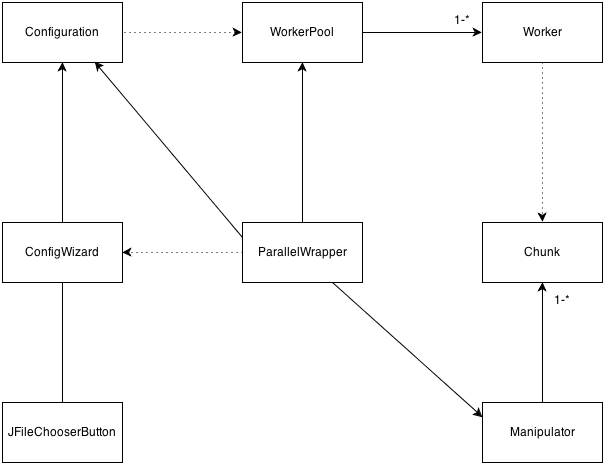
\includegraphics{figures/uml.png}}}
\caption{UML for the embarrassingly parallel framework}
\label{fig:uml}
\end{figure}
The only requirements for a program to be wrapped by framework are that it 
process the input in an embarrassingly parallel manner and that the input comes 
from a file. The processed results must also written to a file. The framework 
supports two forms of input: a directory of files that contain that each contain
one unit of work, which is represented by the Chunk class, or a single file that
the framework can break up into Chunks. For example, the Ka/Ks Calculator's 
input consists of a header and then two protein sequence lines followed by a 
blank line. The framework uses that blank line to know when one Chunk of work 
has ended and another has begun. The user can input a regular expression to 
define when lines of input are separated into Chunks. This occurs in the 
ChunkManager class. 

The other purpose of the ChunkManager class is to combine the resulting Chunks 
back together when the worker threads have finished. Once the work has been
done, all of the separate results are spread across several files. Those results 
must be retrieved and combined to construct the final output file. This output 
file must look the same as the output file would look if the program were run 
serially; the output must come in the same order as the inputs in the input file
and headers may need to be deleted from the separate files and added to the 
combined file. There are two other options if the end-user does not want this 
behavior. They can choose to write their own merger in Java, using the 
CustomMerge class, or write their own script to do the merging. 

As more features are added to the framework and as more programs start to use 
the framework, there are more choices for the end-user to make with regards to 
how they want their program to execute. The number of threads to use, various 
flags for the executable and the statistics output are just a few choice the 
user can make. A start-up wizard is displayed at runtime to systematically allow
the end-user to choose the settings for the run. The ConfigWizard class brings 
the user through this process and creates an instance of Configuration when it 
is completed to save the user's settings, allowing the user to rerun with the
same settings without having to go through the ConfigWizard.

Lastly, the worker threads will keep records during execution. The threads 
records their uptime and the number of pieces of work they execute. The runtime 
for each piece of work is also recorded. This information will be used by us to
evaluate the effectiveness of our approach, but can also provide useful
information the can help a user tine a particular application on a particular
type of input data. The statistics for each thread can be found in the Worker 
subclass and the individual Chunk objects will store their own statistics about 
runtime and size.

\section{Results}

In order to observe how the framework changes the runtime of sequential programs 
when using varying numbers of threads, we designed a simple experiment. The 
Ka/Ks Calculator was run through the framework with ten different samples, each 
containing sixteen units of work. Each sample was run by the framework at five 
different level of numbers of worker threads, starting at 1 and increasing by 
powers of two until the 100\% CPU usage (16 processors). These tests were run
with minimal other activity on the server.

\begin{figure}
{\resizebox{5.2in}{!}{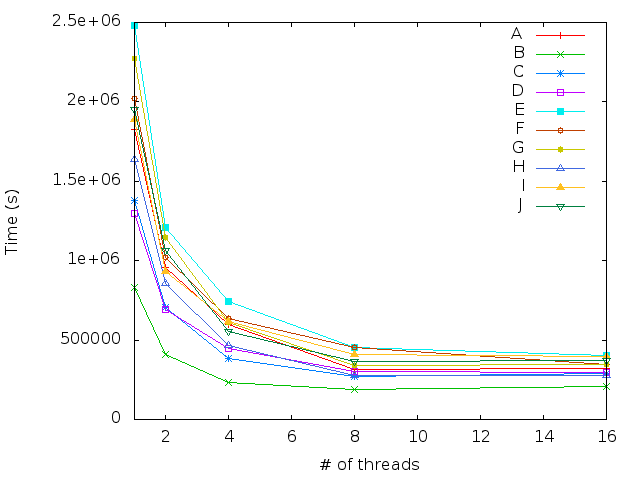
\includegraphics{experiment/out.png}}}
\caption{Runtimes for the Ka/Ks Calculator though the framework}
\label{fig:graph}
\end{figure}

\section{Conclusion}

As the numbers of threads increased, the runtime of the program decreased 
exponentially. In a few cases, there was an increase in time when attempting to 
max out the CPU usage. This occurred because the framework had to wait for the 
CPU to be finished with its previous work before it was allowed to start any 
further jobs. In the cases when the framework executed faster while the CPU was 
maxed out, it was only faster a minute at the most. However, running the 
framework at 50\% of the CPU is more efficient than running using 100\% of the 
CPU. The runtime drop achieved when using 100\% of the CPU versus 50\% is not 
large enough to warrant using all of the machine's power.

Using Java was a good choice for implementation ease and future implementation
extension by others, but it may not produce the fastest results. Languages
like Hadoop, Clojure or other multithread oriented language may have been a
better choice due to their parallel nature. In addition to a single machine 
working to process the data quickly, we can also look to the cloud for help by 
using a networked solution like MPI or a cloud solution like Amazon instances. 
The MapReduce framework works similarly to our framework, there is a step that
splits the data, the Map function is the user's executable and the merge step is
the Reduce function in the framework. In the future, we would like to see this 
work be split into a local front-end and a cloud back-end. This allows for an 
even greater runtime decrease because the number of compute nodes available is 
larger than the number of processors on most machines. Splitting the framework 
also allows for better testing of cloud environments, where the cloud 
environment itself could be a configurable option for end users.

\begin{thebibliography}{1}
\bibitem{history}
Moler, Cleve. ``\emph{Matrix Computation on Distributed Memory Multiprocessors."
}, Hypercube Multiprocessors, 1986: Proceedings of the First Conference on
Hypercube Multiprocessors, Knoxville, Tennessee, August 24-27, 1985. By Michael
T. Heath. Philadelphia: SIAM, 1986. N. pag. Print.
\bibitem{kaks}
Zhang Z, Li J, Zhao XQ, Wang J, Wong GK, Yu J., \emph{Ka/Ks Calculator: 
calculating Ka and Ks through model selection and model averaging},
Genomics Proteomics Bioinformatics, November 2006.
\bibitem{cluster}
Rua, Xu, Wunsch, Donald II, \emph{Survey of Clustering Algorithms},
IEEE Transactions on Neural Networks VOL. 16, NO. 3, MAY 2005
\bibitem{cloud}
Crap, crap and Crap
\end{thebibliography}

\end{document}
